% IEEE ISSRE research-track submission draft (target ~11--12 pages, IEEEtran conference).
% Compile on Overleaf (IEEEtran + IEEEtran.bst are built in). Bibliography: ../refs.bib.
% A local copy of IEEEtran.cls/IEEEtran.bst (V1.8b) is bundled next to this file so the
% paper also compiles offline with a stock TeX Live; on Overleaf the built-in copies are used.
%
% ORIGINALITY NOTE (keep until authorship is final): this paper is built entirely on the
% author's own cross-application study --- the canary-echo method, the six-application
% study (RQ1), the ten-CVE study (RQ2) and the seeded-fault evaluation (RQ3). It does NOT
% claim any course-project deployed-system findings as a contribution.
\IfFileExists{IEEEtran.cls}{\documentclass[conference]{IEEEtran}}{\documentclass[10pt,twocolumn]{article}}
\usepackage{booktabs,amsmath,amssymb,graphicx,xcolor,balance}
\usepackage[hyphens]{url}
\usepackage[final]{microtype}
\usepackage{tikz}
\usetikzlibrary{arrows.meta,positioning,fit,backgrounds,calc}
\usepackage[ruled,vlined]{algorithm2e}
\usepackage{listings}
\lstset{basicstyle=\ttfamily\scriptsize,breaklines=true,columns=fullflexible,
  frame=single,framerule=0.3pt,xleftmargin=2pt,xrightmargin=2pt,
  aboveskip=6pt,belowskip=4pt,captionpos=b,abovecaptionskip=4pt}
\newcommand{\todo}[1]{\textcolor{red}{[TODO: #1]}}
\newcommand{\tool}{\mbox{\textsc{canary-echo}}}
\newcommand{\code}[1]{\texttt{\small #1}}
% >>> REPLACE the URL below with your real public GitHub repository before submission <<<
\newcommand{\repourl}{\url{https://github.com/your-github-id/rag-trust-lab}}

\begin{document}

\title{Isolated at the Route, Leaking Below:\\
Detecting Derived-State Tenant Isolation Failures\\ in Multi-Tenant RAG Applications}

\author{\IEEEauthorblockN{Lisheng Ni}
\IEEEauthorblockA{Independent Researcher\\
Email: 1175235190@qq.com}}

\maketitle

\begin{abstract}
Retrieval-augmented generation (RAG) applications increasingly serve many users from one
shared instance over shared infrastructure: vector collections, lexical indexes, generation and
question caches, and background indexing workers. Access control is enforced at the API
\emph{route}, but the answer a tenant receives is assembled from \emph{derived state} that the
route never inspects. We show that this structural gap produces cross-tenant leaks that
route-level authorization testing---including Broken-Object-Level-Authorization (BOLA) scanning---is
blind to, and we give a black-box method to find them before launch. \emph{Canary-echo
differential testing} plants owner-identifying canary tokens in each tenant's documents, replaces
the chat and embedding models with a deterministic, OpenAI-compatible \emph{echo} service (no GPU,
no API key), and decides isolation with four content-based oracles over user output, LLM prompts,
persisted artifacts, and route-level denials. We organize the failures the method targets into a
taxonomy of six derived-state leak classes (D1--D6). We evaluate along three axes.
\emph{(i)~Cross-application:} across six open-source multi-tenant RAG systems the method surfaces
two independent real cross-tenant leaks beneath correctly authorized routes---a
version-differential derived-layer leak in Open~WebUI and a dynamic reproduction of an unfixed
sharing-authorization CVE in Khoj---alongside correctly-isolating systems, with no false alarms.
\emph{(ii)~Historical:} across ten public isolation CVEs in ten RAG applications, every advisory is
a route-level (D5) authorization bug; the derived-layer classes are absent from the public record.
\emph{(iii)~Effectiveness:} on seeded faults, the method detects all five injected classes with no
false positives, versus $20\%$ for a route-level IDOR scanner and $80\%$ (with a false positive) for
a static key-analysis baseline. The tool, scenarios, adapters, and data are released.
\end{abstract}

\begin{IEEEkeywords}
software reliability, security testing, tenant isolation, retrieval-augmented generation, broken
object-level authorization, metamorphic testing, differential testing.
\end{IEEEkeywords}

\section{Introduction}
\label{sec:intro}
Retrieval-augmented generation (RAG)~\cite{lewis2020rag} has become the default architecture for
knowledge assistants. A user's question is embedded~\cite{reimers2019sbert,karpukhin2020dpr},
matched against an index of document chunks---by dense nearest-neighbor
search~\cite{malkov2020hnsw,johnson2021faiss}, by lexical BM25~\cite{robertson2009bm25}, or by a
fusion of several signals~\cite{cormack2009rrf}---and the retrieved passages are placed in the prompt of a large
language model that composes the answer~\cite{izacard2021fid}. In education, enterprises, and
software-as-a-service products, these assistants are deployed \emph{multi-tenant}: a single instance
serves many users, each with private documents, over shared storage and shared retrieval indexes.

Isolation between tenants is, before it is a security issue, a software \emph{reliability} problem---
and a particularly insidious one. A system that silently returns one customer's confidential document
to another has failed in service, yet every request returns a $200$, no exception is thrown, and the
latency is nominal: the failure produces no observable \emph{event}. It is therefore invisible to
functional tests (each tenant's own queries answer correctly), invisible to health and performance
monitoring (nothing crashes or slows), and invisible even to software-reliability growth models,
which estimate failure intensity and MTBF from an observed failure process and cannot count a failure
that emits no signal~\cite{jia2011mutation}. The defect surfaces only as a correctness property
\emph{across} tenants---a relation between two executions that conventional per-request testing does
not state. This is the defining shape of a \emph{silent} reliability failure (we develop the framing
in Section~\ref{sec:reliability}), and it is the class a dependable multi-tenant service most needs to
exclude, because the damage is irreversible once an answer reaches a user. The OWASP Top~10 for LLM
applications names cross-tenant leakage a first-class risk~\cite{owasp2025llm} and the OWASP API
Security Top~10 ranks broken object-level authorization (BOLA) the top API risk~\cite{owasp2023api};
yet, as we show, the public record contains \emph{no} reported instance of the derived-state failure
mode we study, which suggests it is under-tested rather than absent.

Most security research on RAG studies attacks on the \emph{model and its data}: extraction of
training or context data~\cite{carlini2021extracting,zeng2024ragprivacy}, indirect prompt
injection through retrieved content~\cite{greshake2023indirect}, and knowledge-base
poisoning~\cite{zou2025poisonedrag}. We study a different and, we argue, more mundane but more
pervasive failure: a tenant who is \emph{correctly denied} a document through the API still receives
its \emph{content} through retrieval. This is not a model attack; it is an engineering failure of
isolation in the data path, and it is a reliability defect that should be caught before release.

\subsection{Why it happens}
A RAG request is authorized at the \emph{route}. The question ``may user $u$ read file $f$?'' is
checked by the object-access handler, and if $f$ is not $u$'s, the handler returns a denial. But
the \emph{answer} is not assembled from that handler; it is assembled from \emph{derived state}---a
vector namespace, a lexical index, a generation or question cache, an index cached inside a
background worker---whose keys are chosen for retrieval quality, not for ownership. When that state
is keyed by a resource identifier or a content hash rather than by owner, a request that is
correctly authorized at the route can still pull another tenant's content from beneath it.
Figure~\ref{fig:layers} makes the gap concrete: the direct-object route and the retrieval path
reach the same stored content through \emph{different} code, and only the former consults the owner
check. The cross-tenant leakage literature in cloud computing established long ago that
\emph{sharing infrastructure creates channels the application layer does not
see}~\cite{ristenpart2009cloud,zhang2012crossvm}; RAG re-introduces the same hazard \emph{inside} a
single process, in its retrieval indexes and caches.

\begin{figure}[t]\centering
\resizebox{\columnwidth}{!}{%
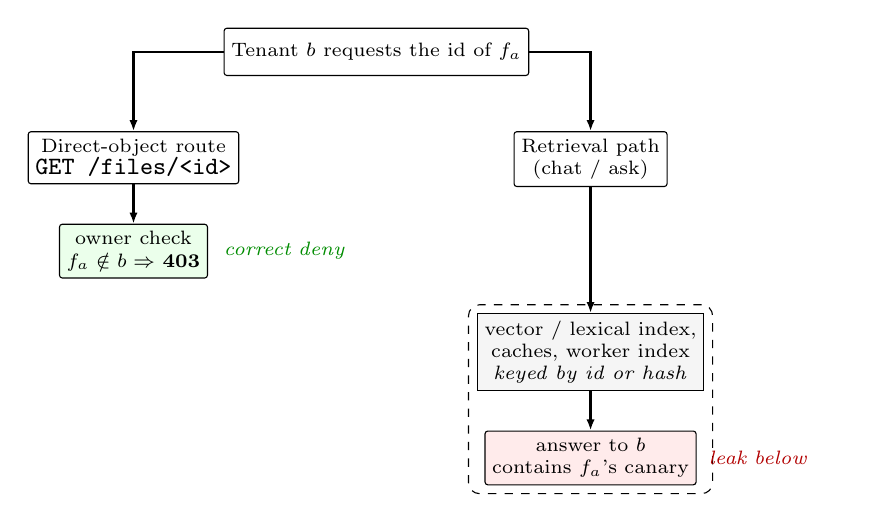
\begin{tikzpicture}[font=\scriptsize,node distance=5.5mm and 7mm,
  box/.style={draw,rounded corners=1pt,align=center,inner sep=2.6pt,minimum height=6.0mm},
  store/.style={draw,align=center,inner sep=2.6pt,minimum height=6.0mm,fill=black!4},
  arr/.style={-{Latex[length=1.4mm]},thick}]
\node[box] (u) {Tenant $b$ requests the id of $f_a$};
\node[box,below left=7mm and -2mm of u] (route) {Direct-object route\\\code{GET /files/<id>}};
\node[box,below right=7mm and -2mm of u] (retr) {Retrieval path\\(chat / ask)};
\node[box,below=5mm of route,fill=green!8] (owner) {owner check\\$f_a\notin b \Rightarrow$ \textbf{403}};
\node[store,below=16mm of retr] (vec) {vector / lexical index,\\caches, worker index\\\emph{keyed by id or hash}};
\node[box,below=5mm of vec,fill=red!8] (ans) {answer to $b$\\contains $f_a$'s canary};
\draw[arr] (u) -| (route);
\draw[arr] (u) -| (retr);
\draw[arr] (route) -- (owner);
\draw[arr] (retr) -- (vec);
\draw[arr] (vec) -- (ans);
\node[right=1mm of owner,text width=18mm,green!55!black] {\emph{correct deny}};
\node[right=0.5mm of ans,text width=18mm,red!70!black] {\emph{leak below}};
\begin{scope}[on background layer]
\node[draw,dashed,rounded corners,fit=(vec)(ans),inner sep=3pt] {};
\end{scope}
\end{tikzpicture}}
\caption{The same stored content is reachable by two paths. The direct-object route consults the
owner check and correctly denies a foreign id; the retrieval path reads from derived state keyed by
id or content hash and never consults it. Route-level authorization testing observes only the left
branch.}
\label{fig:layers}
\end{figure}

\subsection{Why route-level testing misses it}
The mature line of work on authorization testing for web and REST APIs---BOLA/IDOR and
Broken-Function-Level-Authorization detection via fuzzing and specification
analysis~\cite{atlidakis2020checking,corradini2023massassign,santos2025bolapetri,arcuri2025fuzzbola}---operates
at exactly the layer that is implemented \emph{correctly} in these applications. Such tools infer a
violation from an HTTP status code: a request that should be $403$ but returns $200$. But a
derived-layer leak produces a \emph{correct} $403$ on the direct object route and leaks through a
\emph{different} path---retrieval. A status-code oracle at the route cannot see it. We confirm this
empirically in two independent ways: the public CVE record for RAG applications is \emph{entirely}
route-level (Section~\ref{sec:ea2}), and a route-level IDOR scanner detects only one of five
injected leak classes (Section~\ref{sec:ea3}).

\subsection{Approach and contributions}
We make the derived layer observable without a GPU or a paid model. Each tenant's documents carry
\emph{content canaries}: dictionary-compound tokens chosen to survive lexical tokenization as a
single term and to pass through an LLM verbatim; every question additionally carries a per-asker
\emph{query canary}, so that each prompt reaching the model can be attributed to the tenant that
triggered it. The application's chat \emph{and} embedding endpoints are pointed at an \emph{echo}
service---a small OpenAI-compatible server that echoes the canaries it is given, returns deterministic
embeddings so the application's real dense and lexical retrieval still runs, and logs every prompt
with its attributed actor. A leak is then one predicate: a canary owned by tenant $a$ observed in a
context attributed to tenant $b\neq a$. That predicate is a metamorphic, cross-tenant
\emph{differential} relation that canaries make concrete and that sidesteps the generative oracle
problem (developed in Section~\ref{sec:threat}). Our contributions are:
\begin{enumerate}
\item \textbf{Method.} \tool{} differential testing: the first black-box, GPU-free method that makes
the derived layer observable and decides tenant isolation as a two-tenant metamorphic relation
(Section~\ref{sec:method}). A load-bearing design finding is that the route-level denial oracle must
be \emph{content}-based, not status-code based (Section~\ref{sec:oracles}).
\item \textbf{Taxonomy.} Six derived-state leak classes (D1--D6) that name the \emph{keying
mistake} rather than the symptom, with minimal reproducible examples
(Section~\ref{sec:taxonomy}).
\item \textbf{Cross-application study (RQ1).} Six open-source multi-tenant RAG applications; two
independent real-world cross-tenant leaks below correctly authorized routes---a version-differential
derived-layer leak in Open~WebUI and a dynamic reproduction of an unfixed CVE in Khoj---two clean
dynamic negatives, and two opposite source-level verdicts, with no false alarms
(Section~\ref{sec:ea1}).
\item \textbf{Historical study (RQ2).} Ten public isolation CVEs across ten RAG applications, all
route-level (D5), with independent-coder reliability (Section~\ref{sec:ea2}).
\item \textbf{Effectiveness (RQ3).} On seeded faults over $1000$ randomized trials per class, \tool{}
reaches $99.3\%$ aggregate recall (Wilson $95\%$ CI $[99.0\%,99.5\%]$) with zero false positives,
versus $20.0\%$ for route-level IDOR scanning and $80.0\%$ (with a $100\%$ guarded-store false-positive
rate) for static key analysis (Section~\ref{sec:ea3}).
\end{enumerate}
All artifacts---the tool, the scenario suite and adapters, the seeded application, the CVE corpus and
the $\kappa$ coding kit---are released at \repourl, together with a reproducibility guide that
maps every quantitative claim in this paper to the exact command that regenerates it; the
deterministic studies (RQ2's $\kappa$ and all of RQ3, including the $1000$-trial robustness run) are
bit-for-bit reproducible.

\section{Background and Threat Model}
\label{sec:threat}

\subsection{The derived state of a RAG pipeline}
A multi-tenant RAG instance maintains, per tenant or shared across tenants, several pieces of
\emph{derived} state computed from uploaded documents:
\begin{itemize}
\item a \textbf{dense vector index} (an approximate-nearest-neighbor
structure~\cite{malkov2020hnsw,johnson2021faiss}) whose entries map an embedding to a chunk;
\item a \textbf{lexical index} (e.g.\ BM25~\cite{robertson2009bm25}) over the same chunks, often
fused with the dense scores~\cite{cormack2009rrf};
\item \textbf{caches}: a generation cache (answers, summaries), a question or quiz cache, or a
semantic cache keyed by the normalized query or by a content hash;
\item \textbf{in-memory indexes inside worker processes} that serve retrieval and may outlive the
database rows they were built from;
\item \textbf{client-side state} (browser storage) holding chat history or selections.
\end{itemize}
Each is keyed for retrieval efficiency, not for ownership. Correct isolation requires that
\emph{every} such key also scope by owner (or by an owner-bound namespace), and that deletions
propagate to all of them synchronously. The route handler that authorizes \code{GET /files/<id>} has
no visibility into any of these keys, and in general cannot: the indexes are built asynchronously, by
a different component, often in a different process, and are queried by \emph{similarity}, not by
identifier. This is the structural reason the two paths in Figure~\ref{fig:layers} diverge.

\subsection{Isolation as a cross-tenant correctness property}
A convenient way to state the property under test is as a relation over pairs of tenants rather than
over single requests. Let $C(t)$ be the set of content canaries owned by tenant $t$, and let
$\mathsf{obs}(t)$ be the set of canaries observed in any context attributable to $t$---its answers,
the prompts its requests induce, and the artifacts its actions persist. Isolation holds iff, for
every pair $a\neq b$ that are not intentionally sharing,
\[
\mathsf{obs}(b)\cap C(a)=\varnothing .
\]
This is a \emph{safety} property over a two-tenant composition, and it is \emph{metamorphic}: it
constrains the relationship between two executions (tenant $a$'s uploads and tenant $b$'s queries)
rather than the absolute output of either~\cite{chen2018metamorphic,segura2016metamorphic}. Framing
isolation this way is what lets us test a generative system whose single-request output has no
decidable oracle~\cite{barr2015oracle}: we never ask whether $b$'s answer is \emph{correct}, only
whether it contains a token it provably should not.

\subsection{Tenants and adversary}
A \emph{tenant} is an authenticated user who uploads private documents and asks questions answered
over them; tenants may be grouped into workspaces, agents, or shared ``brains,'' and isolation is
expected between tenants that are not intentionally sharing. Our \emph{adversary} is an
authenticated tenant with an ordinary account and no server access, who may (a)~enumerate or reuse
resource identifiers, (b)~place another tenant's resource id on any API that accepts
one---\emph{including the retrieval path}, not only the direct-object route---and (c)~use
otherwise-normal sharing or fork features in unintended combinations. We also consider \emph{benign}
mis-isolation with no adversary at all: identifier reuse after a delete, stale state in a second
worker, or shared-device client storage, each of which can surface one tenant's content to another
with no malice. Out of scope are prompt injection~\cite{greshake2023indirect}, model or
training-data extraction~\cite{carlini2021extracting}, knowledge
poisoning~\cite{zou2025poisonedrag}, and micro-architectural side channels on the serving
infrastructure~\cite{zhang2012crossvm}. We target \emph{isolation of tenant content across the
derived state of the RAG pipeline}.

\section{Canary-Echo Differential Testing}
\label{sec:method}

\subsection{Overview}
The method instantiates the relation of Section~\ref{sec:threat} as an executable differential test.
At a high level (Algorithm~\ref{alg:main}): seed each tenant's documents with owner-tagged canaries;
drive the application through a fixed battery of two-tenant scenarios with its models pointed at the
echo service; collect every observation point (answers, prompts, artifacts, route responses); and
flag any observation attributed to $b$ that contains a canary owned by $a\neq b$. The procedure is
black-box---it needs only the application's ordinary HTTP surface and a configurable model
endpoint---and deterministic, so a flag reproduces.

\begin{algorithm}[t]
\footnotesize
\DontPrintSemicolon
\KwIn{application $A$; tenants $\{a,b,\dots\}$; scenario battery $S$; canary registry $R$}
\KwOut{set of leaks $(\text{owner},\text{observer},\text{oracle},\text{scenario})$}
point $A$'s chat and embedding endpoints at the echo service $E$\;
\ForEach{tenant $t$}{
  create a \emph{regular} (non-admin) account for $t$\;
  \ForEach{document $d$ uploaded by $t$}{seed $d$ with a fresh content canary $c$; $R[c]\gets t$\;}
}
leaks $\gets \varnothing$\;
\ForEach{scenario $s \in S$}{
  execute $s$; each query by $t$ carries $t$'s query canary\;
  \ForEach{observation $o$ attributed to observer $t_o$}{
    \ForEach{canary $c \in o$ with $R[c]\neq t_o$}{
      leaks $\gets$ leaks $\cup\ \{(R[c],\,t_o,\,\mathrm{oracle}(o),\,s)\}$\;
    }
  }
}
\Return leaks\;
\caption{Canary-echo differential isolation test}
\label{alg:main}
\end{algorithm}

\subsection{Canaries}
Each document a tenant uploads is seeded with a \emph{content canary}: a dictionary-compound token
such as \code{OSCARURIAL85}. The design has three requirements. (i)~It must survive \emph{lexical}
tokenization as a single term, so that BM25~\cite{robertson2009bm25} indexes it verbatim---hence a
compound of real dictionary stems rather than random characters, which tokenizers split or drop and
which would therefore become unsearchable through the lexical path. (ii)~It must pass through an
LLM \emph{verbatim}, so that it is recoverable from a generated answer without paraphrase loss.
(iii)~It must be recognizable by a fixed regular expression so that detection needs no per-document
state and no natural-language matching. A registry maps each canary to its owner and its
\emph{kind} (document body, title, metadata), which lets an oracle report not only \emph{that} a
leak occurred but \emph{which} derived field carried it. Every question additionally carries a
per-asker \emph{query canary}; because the asker's query canary accompanies the retrieved context
into the prompt, any prompt reaching the model can be attributed to the single tenant whose query
canary it contains. This attribution is what lets us name the actor of a background job or a
shared-cache generation, where the HTTP request that ultimately surfaces the content may belong to
no one in particular.

\subsection{The echo service}
The application's chat \emph{and} embedding endpoints are configured to a small
OpenAI-compatible \emph{echo} service. For \code{/v1/chat/completions} it returns the canaries
present in the prompt (streaming or non-streaming, matching the client's request), so that
cross-tenant context surfaces in the UI or API exactly as a real model would surface it. For
\code{/v1/embeddings} it returns \emph{deterministic hashing embeddings}, so that the application's
real dense vector search runs and is reproducible and the same canary is reachable by both the dense
and the lexical path. It logs every prompt with its attributed actor. Listing~\ref{lst:echo} shows
the shape of an exchange. The service needs no GPU, no model weights, and no API key; any
application that can point its models at a custom OpenAI-compatible base URL---which is the large
majority of self-hosted RAG systems---can be tested. Deterministic embeddings deliberately trade
retrieval \emph{quality} for \emph{reproducibility}: we are testing which store serves which tenant,
not ranking accuracy, and the canary predicate is independent of embedding fidelity. A real model
would add nondeterminism and cost without changing any oracle's verdict, because the verdict is a
substring test, not a judgment of answer quality.

\begin{figure}[t]
\begin{lstlisting}[caption={An echo exchange. The chat request carries tenant $b$'s query canary and
the retrieved context; the echo service returns the canaries verbatim and logs the prompt under $b$.
If the returned set contains a canary owned by $a$, O-prompt fires.},label={lst:echo}]
POST /v1/chat/completions
{ "messages": [
    {"role":"system","content":"...context: OSCARURIAL85 ..."},
    {"role":"user","content":"...query canary QZB7TENANTB..."} ] }
--> 200
{ "choices": [{"message":{"role":"assistant",
     "content":"echo: OSCARURIAL85 QZB7TENANTB"}}] }
log: actor=tenant_b canaries={OSCARURIAL85(owner=a), QZB7TENANTB(owner=b)}
     => O-prompt LEAK: a-canary in b-attributed prompt
\end{lstlisting}
\end{figure}

\subsection{Oracles}
\label{sec:oracles}
A leak is a canary owned by $a$ observed in a context attributed to $b\neq a$. Four oracles read
different observation points, which matters because an application may suppress a leak at one point
while exposing it at another:
\begin{itemize}
\item \textbf{O-out:} a foreign canary in a user-visible answer---the end-to-end symptom;
\item \textbf{O-prompt:} a foreign canary in an LLM prompt attributed (by query canary) to another
actor---the derived-layer signal, visible even when the UI suppresses the content, and the earliest
point at which the leak is observable;
\item \textbf{O-art:} a foreign canary in a persisted derived artifact (a cache file, an index, an
export) keyed to another owner;
\item \textbf{O-authz:} a route-level request for a foreign resource that nonetheless returns that
resource's content.
\end{itemize}

\paragraph{The route-level oracle must be content-based}
A natural implementation of O-authz is a status-code rule: the attacker's request to a foreign
resource ``passes'' iff it is denied with $401/403/404$, as BOLA fuzzers
assume~\cite{arcuri2025fuzzbola,atlidakis2020checking}. We found this rule unsound in both
directions. Applications signal denial with \emph{different} statuses---$401/403/404$, but also
$400$, and even $200$ with a null body---so a status rule \emph{false-positives} (a $200$-with-null
denial read as a leak) and, more dangerously, \emph{false-negatives} (a $200$ that \emph{does}
return foreign content read as success because its status looked benign). We therefore decide
O-authz by the \emph{same} canary predicate as the other oracles: the attacker passes iff no foreign
canary is returned, and the HTTP status is recorded only for transparency (we tag whether the denial
was a ``hard'' status or a $200$-null). On one correctly-isolating application
(Section~\ref{sec:ea1}) this change removed two spurious failures that a status rule reported, and it
is the single most important robustness decision in the oracle design.

\paragraph{Soundness of the leak signal}
A false positive would require a canary owned by $a$ to appear in $b$'s context \emph{without} any
cross-tenant flow. Because content canaries are high-entropy tokens minted per document and never
reused, and because the matching regular expression admits no natural-language near-misses, the only
way $a$'s canary reaches $b$ is for some component to have served $a$'s derived state to $b$---which
is precisely the failure under test. The signal is therefore dispositive rather than heuristic: a
positive is a proof of leakage, not an anomaly score, and the method reports no severity ranking or
confidence because none is needed. The corresponding risk is a false \emph{negative}---a leak the
scenario battery never triggered---which is why S1 (own-document retrieval) is mandatory: it
certifies that retrieval ran and carried a canary at all, turning an untested path into a visible
gap rather than a silent pass.

\subsection{Scenario suite}
An application-agnostic suite drives one application through a fixed set of scenarios that
systematically stress each keying mistake:
\begin{itemize}
\item \textbf{S1} own-document retrieval---a sanity check that retrieval actually runs and carries
the canary into the prompt; without it a ``clean'' result could be a false negative caused by a
mis-wired adapter rather than by sound isolation;
\item \textbf{S2} explicit cross-ask---a tenant asks for another's content library-wide;
\item \textbf{S3} byte-identical copy for a second tenant---exercises shared caches and
content-addressed sharing (D4);
\item \textbf{S4} delete and re-upload---exercises identifier reuse and stale derived state (D2);
\item \textbf{S5} foreign resource ids on direct-object routes---the BOLA/IDOR surface (D5);
\item \textbf{S6} derived-artifact scan---inspects persisted caches and indexes (D3);
\item \textbf{S7} \emph{derived-layer reference}---the attacker references a victim's raw resource
id \emph{in the retrieval path}, bypassing the direct-object route; this is the class the
route-level tests structurally miss (D1);
\item \textbf{S8} delete-residue---after the victim deletes a resource, the attacker references it
through the derived store (D2/D3);
\item \textbf{P} a prompt audit requiring that every prompt attributed to a tenant contains only
that tenant's canaries---the suite-wide invariant behind O-prompt.
\end{itemize}

\subsection{Adapters and administrator bootstrap}
A per-application \emph{adapter} (typically 80--180 lines) knows only how to create a regular user,
upload a document, ask a question restricted to given resources, delete a resource, substitute
foreign resource ids on direct-object routes, and---optionally---reference a raw resource id in the
retrieval path. Everything else is application-agnostic. Two execution details are load-bearing.
First, test subjects must be \emph{regular} users: an adapter that makes the first account an
administrator by construction would count that account's by-design cross-tenant access as a leak, so
the suite bootstraps a separate non-subject administrator and creates all subjects as regular users.
Second, scenarios that depend on stale worker state (S4/S8, class D2) require retrieval to run
across more than one worker process over a shared store; a single-worker run hides the staleness and
yields a false negative, so the adapter declares the application's worker topology and the harness
provisions accordingly.

\section{A Taxonomy of Derived-State Leaks}
\label{sec:taxonomy}
We name each class by the \emph{keying mistake}, which is what generalizes across applications; the
symptom (which canary surfaces where) varies, the mistake does not. The first four classes (D1--D4)
live in server-side derived state, D5 at the route, and D6 on the client.
\begin{description}
\item[\textbf{D1}] \emph{Owner-less derived index.} A vector or lexical index keyed by resource id
alone (\code{material\_\{id\}}, \code{bm25\_\{id\}}), reachable through retrieval even when the
direct-object API is correct. The route denies; the index does not know there was a question to ask.
\item[\textbf{D2}] \emph{Identifier reuse with stale derived state.} Resource ids recycled---through
delete-and-restore, auto-increment reset, or backup import---while a stale derived index (for
example, inside a second worker that has not reloaded) survives and serves the old content to
whoever now holds the id.
\item[\textbf{D3}] \emph{Release-artifact / orphan cache contamination.} Persisted caches or indexes
shipped inside the release build, or left as orphans after deletes, validated only by a weak
fingerprint such as a chunk count, so that a new tenant's resource is silently matched to a stale
cache entry.
\item[\textbf{D4}] \emph{Content-addressed cross-tenant sharing.} A cache keyed by content hash and
shared across tenants; beyond leaking content, the key doubles as an existence oracle---``has anyone
on this instance uploaded this exact file?''---which is itself a confidentiality breach.
\item[\textbf{D5}] \emph{Client-asserted identity or scope.} Identity or scope taken from the
request body, or ownership checked only \emph{after} the action has run; the route-level class that
BOLA/IDOR testing targets and that fills the public CVE record.
\item[\textbf{D6}] \emph{Client-side persistence across accounts.} Browser storage keyed globally,
so chat history or selections survive logout or an account switch on a shared device.
\end{description}
Our three evaluations show, respectively, that real \emph{public} isolation bugs cluster in D5
(Section~\ref{sec:ea2}); that real D1--D2 leaks nonetheless occur in deployed applications and are
found by our method (Section~\ref{sec:ea1}); and that the method detects all server-side classes
where route-level and static baselines do not (Section~\ref{sec:ea3}). Table~\ref{tab:mre} gives a
minimal reproducible example of each server-side class on a controlled application, each leaking
before and clean after the corresponding fix---evidence that the classes are not merely conceptual
but each correspond to a concrete, independently repairable defect.

\begin{table}[t]\centering\small
\caption{Seeded minimal reproducible examples: each class leaks before its fix and is clean after.}
\label{tab:mre}
\begin{tabular}{@{}l p{5.0cm} cc@{}}
\toprule
Class & Keying mistake (seeded) & Vuln. & Fixed \\
\midrule
D1 & owner-less derived index (id only)        & leak & clean \\
D2 & identifier reuse, stale worker index       & leak & clean \\
D3 & shipped / orphan cache, weak fingerprint   & leak & clean \\
D4 & content-hash cache shared across tenants   & leak & clean \\
\bottomrule
\end{tabular}

\end{table}

The D1 mistake is instructive because it is a one-token omission that no route test can
observe. Listing~\ref{lst:d1} contrasts a vulnerable owner-less retrieval query with its
owner-scoped fix: the direct-object route above it may be flawless, yet the query beneath it reaches
every tenant's chunks. The repair is to add the owner predicate to the \emph{retrieval} filter, not
only to the route---and the only way to know it was missing, short of reading every query, is to
observe that a foreign canary came back.

\begin{figure}[t]
\begin{lstlisting}[caption={D1 in one line. The retrieval query selects chunks by resource id alone
(top); the fix (bottom) scopes the same query by owner. The direct-object route is unchanged and
may be correct in both cases.},label={lst:d1}]
# vulnerable: owner-less derived index (D1)
chunks = index.search(embedding, where={"source_id": sid})

# fixed: owner-scoped retrieval filter
chunks = index.search(embedding,
    where={"source_id": sid, "owner": current_user.id})
\end{lstlisting}
\end{figure}

\section{RQ1: Cross-Application Study}
\label{sec:ea1}
\emph{RQ1: Does the method find real derived-state isolation failures in deployed open-source RAG
applications, without false alarms on correctly isolating ones?}

\subsection{Setup}
We selected six open-source multi-tenant RAG applications spanning distinct architectures and vector
stores, each self-deployed in isolation on hardware we control, with its chat and embedding models
pointed at the echo service. Four expose an HTTP API sufficient to drive the suite dynamically; two
do not---one is a Gradio-only application with no stable REST surface, and one is a four-container
RAG stack whose memory footprint exceeded our isolated test host---and for those two we confirm the
isolation property at the source level against the exact released revision, reading the ownership
predicate on every path that reaches the derived store. Every dynamic finding is accompanied by a
positive control (a configuration or version known to leak) and a negative control (one known to be
sound), so that a ``leak'' verdict is never an artifact of a mis-wired adapter and a ``clean''
verdict is never the silent failure of a test that never exercised retrieval.
Table~\ref{tab:apps} lists the six applications and the axes along which they differ---interface,
vector store, and the unit over which tenancy is defined---and Table~\ref{tab:ea1} summarizes the
results. The spread matters: a method that generalizes must work across a shared single collection
(Open~WebUI), per-namespace stores (AnythingLLM), a relational pgvector backend (Khoj, LibreChat),
and a tenancy unit that is sometimes a user, sometimes a workspace, and sometimes an agent.

\begin{table}[t]\centering\small
\setlength{\tabcolsep}{4pt}
\caption{The six applications under study and the axes along which they differ.}
\label{tab:apps}
\begin{tabular}{@{}l l l l@{}}
\toprule
Application & Interface & Vector store & Tenancy unit \\
\midrule
Open~WebUI & REST & shared collection & user \\
Khoj & REST (Django) & pgvector & user / agent \\
AnythingLLM & REST & per-workspace ns & workspace \\
LangFlow & REST & per-user store & user \\
Kotaemon & Gradio only & local index & user \\
LibreChat & REST + RAG svc & pgvector (svc) & user \\
\bottomrule
\end{tabular}
\end{table}

\begin{table*}[t]\centering\footnotesize
\setlength{\tabcolsep}{4pt}
\caption{RQ1 cross-application results. ``Dyn.''~=~driven dynamically over HTTP; ``Src''~=~source-level confirmation against the released revision.}
\label{tab:ea1}
\begin{tabular}{llll p{9.2cm}}
\toprule
Application & Mode & Layer & Verdict & Finding \\
\midrule
Open~WebUI & Dyn. & route + derived & \textbf{leak (D1,\,D2)} & A regular user reads a foreign file's content via the chat file-reference path (S7) and via delete-residue in the shared vector store (S8), while the direct file API returns $404$ for the same id (S5 passes). Present in 0.8.11, absent from 0.10.2 onward. \\
Khoj & Dyn. & route + derived & \textbf{leak (D5$\rightarrow$KB)} & CVE-2026-13508 (fix PR unmerged): a user forks a publicly shared conversation and obtains one bound to the author's \emph{private} agent; the app's own agent-access predicate returns false for the forker, yet the agent's knowledge base holds the author's canary, which the chat retrieval selects via an agent-scoped filter with no user bound. \\
AnythingLLM & Dyn. & route + derived & clean & Per-workspace vector namespace plus membership-checked chat; cross-workspace access is denied (via $200$-null / $400$ / $404$) with no content leak. \\
LangFlow & Dyn. & route (object) & clean & Cross-user object access returns $404$; no content leak on any path the adapter exercises. \\
Kotaemon & Src & route + derived & \textbf{leak (D5, unfixed)} & CVE-2026-82281 (unfixed at HEAD): four conversation handlers fetch by id with no owner predicate (the sibling history loader has one); retrieval additionally selects by \code{source\_id} alone, a latent D1 surface. \\
LibreChat & Src & route + derived & clean & Message-referenced files are admitted only from an owner-scoped map (\code{\{file\_id, user\}}) and the RAG service filters by a per-user token; a foreign \code{file\_id} is dropped before retrieval. Its historical credential-IDOR CVE is fixed. \\
\bottomrule
\end{tabular}
\end{table*}

\subsection{Flagship case: Open~WebUI (version-differential)}
On a pinned vulnerable image (0.8.11) the suite's checks fail at exactly two points. In \textbf{S7},
a regular user supplies a \emph{foreign} \code{file\_id} in the chat request's file-reference list;
the retrieval path loads that file's content and places it into the attacker's own prompt, where the
victim's content canary appears (O-prompt and O-out both fire). In \textbf{S8}, after the victim
\emph{deletes} the document, its entries in the shared vector collection are not purged and remain
retrievable by another user. Crucially, the \emph{route-level} checks (S5) \emph{pass}: the same user
calling \code{GET /files/<id>} on the victim's id is correctly denied with $404$. This is the
pattern the paper is named for---isolated at the route, leaking below. A pinned \emph{fixed} image
(0.12.5) passes all checks, a clean negative control, and a role-aware positive control reproduces
the application's public route-level CVE so that we know the harness can see a leak when one exists.

A version bisection localizes the derived-layer fix to the interval $(0.8.11,\,0.10.2]$, consistent
with the vendor's stated fix release. The intermediate 0.9.5 is \emph{not} adjudicable by this oracle
because its file-reference endpoint rejects \emph{any} file reference---own or foreign---with a
server error, which an own-file control (S1) confirms is an API change rather than an ownership
check. Reporting that honestly, rather than scoring 0.9.5 as ``fixed,'' is exactly the kind of
control the canary oracle makes cheap: because S1 distinguishes ``retrieval is off'' from ``retrieval
is isolated,'' we avoid crediting a sound verdict to what is really a broken endpoint.

\subsection{Second positive: Khoj (a live, unfixed CVE)}
Using only documented REST endpoints, tenant $B$ forks a conversation that tenant $A$ shared
publicly and thereby obtains a conversation \emph{bound to $A$'s private agent}: the fork copies the
agent with no access check. We confirm the leak with the application's own code: Khoj's
authorization predicate \code{ais\_agent\_accessible(agent, B)} returns \code{False}---the check the
fork-then-chat path omits---while the agent's knowledge base holds $A$'s private canary, which the
chat retrieval selects with \code{user=None} and \code{owner\_filter=Q(agent)}. A control in which
$B$ chats without the forked agent sees nothing of $A$'s, so the leak is specific to the asymmetric
share/fork$\rightarrow$agent-knowledge path, not to personal documents. We note a method limitation
here: the full chat-level answer could not be elicited with the deterministic echo backend, because
Khoj's pipeline uses the model itself to decide \emph{whether and what} to retrieve, and the echo
service does not satisfy those intermediate structured decisions; we therefore confirm at the
retrieval/authorization layer using the application's real code rather than overclaiming a UI-level
reproduction. This case shows both the reach of the method (it localized a live, unfixed
cross-tenant leak) and an honest boundary of the echo technique (Section~\ref{sec:threats}).

\subsection{Clean negatives and precision}
AnythingLLM and LangFlow isolate correctly and produce \emph{no} false alarms. AnythingLLM is the
case that motivated the content-based O-authz oracle (Section~\ref{sec:oracles}): it denies
cross-workspace access with $200$-plus-null and $400$ responses that a status-code rule flags as
leaks even though no canary is ever returned. With the content-based oracle, all of its checks pass,
and the two spurious failures disappear. That a precision fix on one application is driven by an
observation on another is itself an argument for a uniform, content-based oracle rather than a
per-application status allowlist.

\subsection{Source-level confirmations}
Kotaemon, a Gradio-only application without a REST surface, is confirmed \emph{positive} by source
against its released revision: four conversation handlers fetch a conversation by id with no owner
predicate, in contrast to a sibling history loader that filters by owner---an unfixed CVE---and the
retrieval query selects chunks by \code{source\_id} alone, a latent owner-less-index (D1) surface.
LibreChat, a four-container RAG stack, is confirmed \emph{negative}: a message-referenced file is
admitted only if present in an owner-scoped map, the agents path loads attachments with a
user-scoped query, and the retrieval service additionally filters by a per-user token, so a foreign
\code{file\_id} is dropped before it reaches retrieval; its historical credential-IDOR is fixed in
the current release. The two opposite source-level verdicts show the taxonomy discriminates in both
directions, not only toward ``leak,'' and that the method's negative verdicts are falsifiable claims
about specific predicates in specific code, not an absence of evidence.

\subsection{Answer to RQ1}
The method found two independent real-world cross-tenant leaks beneath correctly authorized routes
(one a version-differential derived-layer leak, one a live unfixed CVE), returned clean negatives on
two correctly-isolating applications with no false alarms, and produced two opposite verdicts at the
source level. In every positive case the route-level checks passed while the derived-layer checks
failed---the precise gap route-level testing cannot observe.

\section{RQ2: What the Public Record Contains}
\label{sec:ea2}
\emph{RQ2: Are derived-state isolation bugs represented in the public vulnerability record for RAG
applications, and how reliably can isolation bugs be classified into D1--D6?}

\subsection{Corpus and method}
We assembled, from OSV, the NVD, and GitHub Security Advisories, one public isolation CVE for each of
ten open-source RAG applications, verifying each against its authoritative advisory and, where a fix
exists, against the upstream repository (tag, merge-base, or fix pull request). During verification
we corrected a subtlety that matters for honesty: for three applications the identifier recorded by
aggregators as the ``fixed'' commit is a \emph{release} commit (a version bump) rather than the
granular security patch, so we report the fixed \emph{version} and do not attribute a specific
line-level fix we did not confirm. We then classified each CVE into D1--D6.
Table~\ref{tab:incidents} lists the corpus.

\begin{table}[t]\centering\small
\caption{RQ2: ten public isolation CVEs; every one is a route-level (D5) class. ``---''~=~no released fix at the time of writing.}
\label{tab:incidents}
\begin{tabular}{llcl}
\toprule
Application & CVE & CWE & Fixed \\
\midrule
Open~WebUI & 2026-45402 & 639 & 0.9.5 \\
AnythingLLM & 2026-55611 & 639 & 1.14.1 \\
Dify & 2026-34082 & 284/863 & 1.13.1 \\
RAGFlow & 2026-51892 & 284 & --- \\
LibreChat & 2026-31942 & 862 & 0.8.3-rc1 \\
Kotaemon & 2026-82281 & 639 & --- \\
Onyx & 2024-7767 & 862 & --- \\
FastGPT & 2026-61644 & 863 & 4.15.0-beta5 \\
Khoj & 2026-13508 & 285/863 & --- (PR open) \\
Quivr & 2026-82280 & 639 & --- \\
\bottomrule
\end{tabular}
\end{table}

\subsection{Finding: the public record is entirely route-level}
All ten advisories are route-level object- or function-authorization bugs (D5):
CWE-639 (authorization bypass through a user-controlled key, $\times4$), CWE-862 (missing
authorization, $\times2$), CWE-863 (incorrect authorization), CWE-284, CWE-285, and combinations.
\emph{Not one} is a derived-layer (D1--D4) leak. We read this not as a sampling artifact but as the
result: public advisories record authorization bugs that can be demonstrated in a single route call
and mapped cleanly to a CWE, which is precisely where route-level BOLA
testing~\cite{arcuri2025fuzzbola,corradini2023massassign,santos2025bolapetri} and the broader
REST-API-testing literature~\cite{atlidakis2019restler,golmohammadi2023survey,zhang2023openproblems}
are strong. Derived-state leaks keyed by identifier, content hash, or stale index are systematically
\emph{absent}. The one public case that touches a derived index is an id-manipulation that
\emph{poisons} another tenant's index---a write reached through a route-level flaw, aligned with
knowledge-poisoning attacks~\cite{zou2025poisonedrag}, not the cross-tenant \emph{read} our method
surfaces. A second observation on the disclosure landscape: only five of the ten carry a released
fix; the others are unpatched, carry an open fix pull request, or had the vulnerable code removed
only incidentally in a later rewrite---so these are not merely historical curiosities but a live
state of the ecosystem.

\subsection{Classification reliability}
Reliability of a manual taxonomy is standard to report with an inter-coder agreement
coefficient~\cite{cohen1960kappa,landis1977kappa}. One author and an \emph{independent LLM
annotator}---given only the codebook and neutral one-line descriptions, with no project context and
no sight of the author's labels---classified a mixed set of thirteen cases (the ten route-level CVEs
plus three derived-layer cases: our two Open~WebUI findings and the public index-poisoning case). A
single-category set would make $\kappa$ degenerate (observed and expected agreement both $1$), so the
derived-layer cases are included deliberately to give the scale range. Agreement on the ten
route-level CVEs was $100\%$ (both assigned D5 to all ten); over the full set Cohen's
$\kappa=0.46$ (moderate on the Landis--Koch scale~\cite{landis1977kappa}). All disagreement fell on
the two cases at the route-vs-derived boundary, where the annotator read an id-manipulation framing
as route-level and the author read the ``direct API denies, retrieval leaks'' framing as
derived-layer---the very subtlety that makes these leaks easy to overlook, and that motivates a
testing method rather than a classification exercise. We disclose that the second annotator is an
LLM, not a human expert; human replication is a stronger follow-up, and the blind coding materials
are released for it.

\section{RQ3: Effectiveness on Seeded Faults}
\label{sec:ea3}
\emph{RQ3: On faults of known class, how does the method's detection compare to route-level IDOR
scanning and to static key analysis?}

\subsection{Setup}
Seeding faults of a known class to measure a detector's effectiveness is the standard fault-injection
methodology used throughout mutation and reliability testing~\cite{jia2011mutation}. We built a
controlled RAG application into which one fault of each class D1--D5 can be injected independently,
plus a \emph{clean} configuration and a \emph{guarded-but-owner-less} configuration---a derived store
keyed without an owner component but protected by a correct runtime ownership check, which is a
deliberate false-positive trap for static analysis. We ran three detectors: \tool{} (ours); a
\emph{route-level IDOR scanner} that substitutes foreign resource ids on direct-object routes and
flags a non-denied response, as BOLA fuzzers
do~\cite{arcuri2025fuzzbola,corradini2023massassign}; and a \emph{static key-analysis} baseline that
flags any derived store whose key lacks an owner component.

Table~\ref{tab:ea3} reports the canonical single-fault result. To answer the obvious objection that a
single injection per class yields no estimate of stability, we additionally ran a
\textbf{multi-seed robustness study}: for each configuration we executed $N{=}1000$ \emph{independent
randomized trials}, each drawing a fresh realization of the fault---different canary tokens, different
document content (section count, marker positions, vocabulary), a different benign-document
realization, and a randomized worker count ($2$--$4$)---and ran the same three detectors on it. This
yields $5000$ class-trials per detector; Table~\ref{tab:ea3ms} reports per-class detection rate and a
Wilson $95\%$ confidence interval on each detector's aggregate recall.

\begin{table}[t]\centering\small
\setlength{\tabcolsep}{3.5pt}
\caption{RQ3 canonical single-fault result: detection of five seeded classes and false positives (FP).}
\label{tab:ea3}
\begin{tabular}{lccccc c c}
\toprule
Detector & D1 & D2 & D3 & D4 & D5 & Recall & FP \\
\midrule
\tool{} (ours) & \checkmark & \checkmark & \checkmark & \checkmark & \checkmark & $100\%$ & 0 \\
IDOR scanner & & & & & \checkmark & $20\%$ & 0 \\
Static keying & \checkmark & \checkmark & \checkmark & \checkmark & & $80\%$ & 1 \\
\bottomrule
\end{tabular}
\end{table}

\begin{table}[t]\centering\small
\setlength{\tabcolsep}{2.6pt}
\caption{RQ3 multi-seed robustness: $N{=}1000$ independent randomized trials per configuration ($5000$ class-trials per detector). Per-class detection rate (\%) and aggregate recall with Wilson $95\%$ CI. ``FP$_g$''~=~false-positive rate on the guarded-but-owner-less store.}
\label{tab:ea3ms}
\begin{tabular}{@{}lccccc c c@{}}
\toprule
Detector & D1 & D2 & D3 & D4 & D5 & Recall (95\% CI) & FP$_g$ \\
\midrule
\tool{} & 99 & 99 & 98 & 100 & 100 & \textbf{99.3} [99.0,99.5] & 0 \\
IDOR & 0 & 0 & 0 & 0 & 100 & 20.0 [18.9,21.1] & 0 \\
Static & 100 & 100 & 100 & 100 & 0 & 80.0 [78.9,81.1] & 100 \\
\bottomrule
\end{tabular}
\\[2pt]
\footnotesize Per-class values are detection rate (\%); recall and CI in \%; FP$_g$ in \%.
\end{table}

\subsection{Finding}
\tool{} detects all five classes with no false positive in the canonical run, and the robustness
study confirms the result is stable, not a lucky seed: aggregate recall is $99.3\%$ (Wilson $95\%$ CI
$[99.0\%,99.5\%]$) over $5000$ randomized class-trials, with per-class detection $98$--$100\%$ and a
false-positive rate of $0\%$ on both the clean and the guarded-but-owner-less app across all $1000$
trials. The handful of misses are confined to D2 and D3 and trace to the finite per-trial probe
budget occasionally not scheduling a query onto the stale worker index or not ranking the
contaminated chunk into the top-$k$ under an adversarial random document---a \emph{probe-coverage}
limit, not an oracle error (the content oracle never once fired on content that had not crossed
tenants). The IDOR scanner is pinned at $20.0\%$ ($[18.9\%,21.1\%]$): it exercises the route layer,
which is exactly where D1--D4 are not; this is the same blind spot we observed in Open~WebUI (RQ1),
where the route checks passed while the derived-layer checks failed, and in the public record (RQ2),
which is entirely D5. Static key analysis is pinned at $80.0\%$ ($[78.9\%,81.1\%]$): it detects the
four derived-layer classes but misses D5---a route-level mistake over correctly-keyed storage,
invisible to a key-shape rule---and \emph{false-positives on every one} of the $1000$ guarded-but-%
owner-less trials, because it cannot see the runtime guard. The separation between the three detectors
is therefore not a within-noise artifact: the confidence intervals do not overlap, and each baseline
is blind to a region the dynamic, content-based method covers. In practice a team would run
route-level BOLA testing \emph{and} \tool{}; the point of RQ3 is that neither the route scanner nor
static analysis is a substitute for observing the derived layer dynamically.

\section{Discussion}

\subsection{Isolation failure as a reliability defect}
\label{sec:reliability}
We have framed cross-tenant leakage as a security issue, but it is first a \emph{dependability}
failure, and treating it as one explains why it survives conventional assurance. A multi-tenant
service makes an implicit correctness contract---each tenant's answers are computed only from that
tenant's authorized data---and a derived-state leak violates that contract silently: the request
succeeds, the status is $200$, no exception is raised, and the latency is nominal. Three standard
reliability instruments therefore cannot see it. Functional tests pass, because each tenant's own
queries return correct answers; the defect is only visible in the \emph{relation} between two
tenants' executions, which single-execution test cases do not state. Runtime health monitoring is
silent, because there is no crash, error rate, or latency excursion to alarm on---the failure has no
observable \emph{event}. And software-reliability growth models, which estimate failure intensity and
MTBF from an observed failure process~\cite{jia2011mutation}, cannot estimate the intensity of a
failure that produces no signal to count; a system can leak on a large fraction of cross-tenant
interactions while its measured failure intensity is zero. This is the defining shape of a
\emph{silent} correctness failure, and it is precisely the class a dependable multi-tenant system
most needs to exclude, because the damage---one tenant's confidential corpus surfacing in another's
answer---is irreversible once it reaches a user and erodes the trust assumption on which the shared
deployment rests. Our contribution, read in reliability terms, is to give this silent failure an
\emph{observable} proxy (the canary predicate) and a \emph{differential} test case form (the
two-tenant metamorphic relation), turning a property that growth models cannot measure into one a
fault-injection study can quantify---which is exactly what RQ3's recall-with-confidence-interval
does. The method extends reliability testing to a correctness property that the usual failure-event
machinery misses, rather than merely porting a security scanner.

\paragraph{Why route-level testing is necessary but not sufficient}
RQ2 shows the public record is entirely route-level; RQ1 and RQ3 show that derived-layer leaks
nevertheless occur and that neither IDOR scanning nor static key analysis catches the whole picture.
BOLA/IDOR testing~\cite{arcuri2025fuzzbola,corradini2023massassign,santos2025bolapetri} remains
essential---D5 is real and common, and tops the OWASP API list~\cite{owasp2023api}---but isolation
testing for RAG must additionally observe the derived layer, which is what the echo service and the
O-prompt/O-art oracles do. The two lines are complementary, not competing: a complete pre-launch
check runs both, and our seeded-fault study quantifies exactly what each misses.

\paragraph{Closest baseline, made concrete}
The nearest prior work is the addition of BOLA/BFLA oracles to a REST
fuzzer~\cite{arcuri2025fuzzbola}: for a resource owned by $a$, the fuzzer replays $a$'s request as
$b$ and flags a violation when the response status is not a denial ($401/403$). This is the right
test for D5 and we do not improve on it there. The difference is the observation point and the
decision rule. Their oracle reads the \emph{status} of the \emph{direct-object} response; ours reads
the \emph{content} of \emph{every} observation point, including the LLM prompt and persisted
artifacts that the direct-object route never produces. Concretely, on the Open~WebUI leak (RQ1) a
status-BOLA oracle sees \code{GET /files/<id>}~$\to$~$404$ and correctly concludes the route is
sound---and stops, because it has no notion of a retrieval path that re-reads the same file by id.
Our oracle additionally issues the chat request that carries the foreign id into retrieval and
observes $a$'s canary in $b$'s prompt. The two oracles agree on D5 and diverge exactly on D1--D4,
which is why RQ3 reports $20\%$ recall for the status oracle and $100\%$ for ours: not because the
status oracle is wrong about what it tests, but because the derived layer is outside what it tests.
Symmetrically, the content rule repairs a precision problem the status rule has even at the route
(the AnythingLLM $200$-null denials of RQ1), so the content-based decision dominates the status-based
one on both recall and precision.

\paragraph{Generality and cost}
The method applies to any RAG application that can point its chat and embedding models at a custom
OpenAI-compatible endpoint, which covers the large majority of self-hosted systems. Adding an
application costs one adapter (80--180 lines); the canary and oracle design is independent of the
vector store, the embedding model, and the LLM, and the echo service runs on a CPU with no API key,
so a full run of the suite is a matter of minutes and dollars-free. This cost profile matters for a
reliability practice: a check cheap enough to run on every release is one that will actually be run.

\paragraph{Operational integration}
Because the suite is black-box and deterministic, it fits an ordinary continuous-integration stage:
spin up the application under test with its model endpoints pointed at the echo service, run the
adapter and scenario battery, and fail the build on any non-empty leak set. The owner-tagged canary
registry makes each failure self-describing---owner, observer, oracle, and scenario---so a
regression points directly at the derived store that leaked rather than at a generic assertion
failure. A team adopting the method incrementally can begin with S1, S5, and S7 (own-document
sanity, the route surface, and the derived-layer reference), which together already separate ``route
correct, derived layer leaking'' from ``both correct,'' and add the remaining scenarios as their
worker topology and caching layers warrant. The determinism is what makes this practical: a
flaky isolation test that fails once in ten runs would be disabled within a sprint, whereas a
substring predicate over echoed canaries either fires or does not.

\subsection{Threats to validity}
\label{sec:threats}
\paragraph{Construct}
Deterministic echo embeddings are not the application's production model; we test the \emph{plumbing}
of isolation (which store serves which tenant), not retrieval quality, and the canary predicate does
not depend on embedding fidelity. One construct limitation is concrete: applications whose pipeline
uses the model to decide whether and what to retrieve (observed in Khoj) cannot be driven end-to-end
by a trivial echo; for those we confirm at the retrieval/authorization layer with the application's
own code, and a retrieval-planning-aware mock LLM is future work.

\paragraph{Internal}
Every dynamic finding has a positive and a negative control (a vulnerable vs.\ a fixed version, or a
leaking vs.\ a guarded configuration), and the S1 own-document check guards against crediting a
``clean'' verdict to an adapter that never exercised retrieval. Test subjects are always regular
users; the suite bootstraps a separate administrator so that by-design administrative access is not
miscounted. Route-level denial is judged by content, not status code, removing a class of false
positives demonstrated on AnythingLLM (RQ1).

\paragraph{External}
Six applications are not the ecosystem, and two were confirmed only at the source level; broadening
the dynamic set is the main threat to external validity. The seeded-fault study, by contrast, is now
backed by $1000$ randomized trials per class with reported confidence intervals
(Section~\ref{sec:ea3}), so its effectiveness claim is not a single-seed artifact; its remaining
limitation is that the seeded application is a controlled model of the five server-side mechanisms
rather than production code, so its absolute recall need not transfer verbatim to a specific system,
even though the \emph{separation} between detectors is robust. The historical corpus is one CVE per
application; a census of \emph{all} isolation CVEs per application would sharpen the ``derived layer
is absent'' claim. The inter-coder study uses an LLM as the second annotator; human replication is
the stronger form, and the materials are released for it.

\paragraph{Ethics and responsible disclosure}
All tests ran against self-deployed, isolated instances only; no third-party or production service
was touched, and the released artifacts drive only local deployments. Every real-world finding is
either an already-public CVE or a leak fixed in the current release, so we introduce no new
undisclosed vulnerability; for the one live, unfixed CVE (Khoj) we rely on the vendor's existing
public advisory and open fix pull request, and add no exploitation detail beyond what is needed to
substantiate the classification.

\section{Related Work}
\label{sec:related}
\paragraph{RAG and LLM security}
Work on RAG security has centered on attacks against the model and its data: extraction of training
or context data~\cite{carlini2021extracting,zeng2024ragprivacy}, direct and indirect prompt
injection through retrieved content~\cite{greshake2023indirect,liu2024promptinject}, and
knowledge-base poisoning~\cite{zou2025poisonedrag}; the OWASP LLM Top~10 names vector/embedding
weaknesses as a category~\cite{owasp2025llm}. These study how an adversary manipulates \emph{what the model knows or
says}. We study whether a deployed application's \emph{derived state} already leaks one tenant's
documents to another, independent of any model attack---a question about the engineering of
isolation, not about the model.

\paragraph{Authorization testing for web and REST APIs}
There is a mature line on testing authorization in REST APIs. General REST fuzzers and test
generators---RESTler~\cite{atlidakis2019restler}, EvoMaster~\cite{arcuri2019evomaster},
RestTestGen~\cite{viglianisi2020resttestgen}, RESTest~\cite{martinlopez2021restest},
Morest~\cite{liu2022morest}, MINER~\cite{lyu2023miner}, NAUTILUS~\cite{deng2023nautilus},
ARAT-RL~\cite{kim2023aratrl}, VOAPI2~\cite{du2024voapi2}, and tools examined in recent surveys,
comparisons, and coverage
studies~\cite{golmohammadi2023survey,zhang2023openproblems,kim2022notime}---maximize
schema and code coverage and detect faults chiefly via server-error (5xx) status codes.
Security-focused extensions check authorization specifically: Atlidakis et al.\ check security
properties including resource-after-delete and cross-namespace access~\cite{atlidakis2020checking};
Corradini et al.\ detect mass-assignment vulnerabilities~\cite{corradini2023massassign}; Du et al.\
target vulnerability-oriented testing~\cite{du2024voapi2}; Santos~Filho et al.\ detect broken
object-level authorization by transforming OpenAPI specifications to colored Petri
nets~\cite{santos2025bolapetri}; and, most closely to us, Arcuri et al.\ add automated oracles for
access-policy violations (BOLA/BFLA) to a REST fuzzer, inferring violations from $401/403$
responses~\cite{arcuri2025fuzzbola}. All of these operate at the \emph{route}: they decide
authorization from the direct-object response and its status code. Our contribution is orthogonal and
complementary---we observe the \emph{derived state} beneath a correctly authorized route, and we show
(RQ1, RQ3) that a status-based route oracle both misses derived-layer leaks and misclassifies
non-standard denials. Policy-coverage and access-control-policy
testing~\cite{barr2006policycoverage,fisler2005verification} similarly reason about the specified
policy, not about derived indexes that no policy mentions.

\paragraph{Metamorphic, differential, and oracle-free testing}
Our oracle is a metamorphic relation---``tenant $a$'s content must not appear for tenant
$b$''~\cite{chen2018metamorphic,segura2016metamorphic}---instantiated concretely by canaries and
evaluated \emph{differentially} across tenants~\cite{mckeeman1998differential}. Metamorphic security
testing has been applied to web systems~\cite{mai2020metamorphic}; we specialize it to RAG tenant
isolation, where the generative component makes a direct correctness oracle
impractical~\cite{barr2015oracle} and a canary-based relation sidesteps it. Fuzzing more
broadly~\cite{manes2021fuzzing} shares our black-box, input-generation stance but relies on crash or
coverage oracles that do not capture cross-tenant content flow, which is a functional-correctness
property rather than a memory-safety one.

\paragraph{Multi-tenant isolation}
Cross-tenant information leakage on shared infrastructure is a long-standing concern in cloud
computing~\cite{ristenpart2009cloud,zhang2012crossvm}; those leaks exploit shared hardware beneath
the application, whereas ours arise \emph{inside} a single application's retrieval indexes and
caches. The hazard---sharing state keyed for efficiency rather than for ownership---is the same; the
layer and the remedy differ, and the RAG setting adds a new twist: the leaking channel is the
application's \emph{intended} retrieval path, not an unintended side channel.

\section{Conclusion}
Isolation in multi-tenant RAG is enforced where it is easy to see, at the API route, and fails where
it is not, in the derived state---vector namespaces, lexical indexes, caches, and worker
indexes---that assembles the answer. \tool{} differential testing makes that layer observable with
owner-identifying canaries and a deterministic, GPU-free echo service, and decides leaks with four
content-based oracles over a metamorphic cross-tenant relation. Across six open-source applications
it finds two independent real leaks beneath correct routes with no false alarms; across ten public
CVEs it shows that the derived layer is absent from the record while route-level bugs fill it; and on
seeded faults it detects every server-side class that route-level and static baselines miss. The
derived layer is where multi-tenant RAG leaks---and, with the right canaries and oracles, it is
testable before launch.

Several directions would strengthen the method and the evidence. A retrieval-planning-aware mock
model---one that satisfies the structured intermediate decisions a pipeline like Khoj's makes, while
still echoing canaries deterministically---would let the echo technique drive end-to-end answers in
applications that currently require source-level confirmation. On the empirical side, a human second
annotator would replace the LLM-based inter-coder measurement, a census of \emph{all} isolation CVEs
per application (rather than one representative each) would test the ``derived layer is absent from
the public record'' claim at larger scale, and multiple independent seeds per fault class would put
confidence intervals on the RQ3 recall figures. Finally, partial synthesis of adapters from an
application's OpenAPI description would lower the per-application cost further and make
derived-state isolation testing a routine part of every RAG release.

\balance
\bibliographystyle{IEEEtran}
\bibliography{../refs}
\end{document}
